% -*- coding: utf-8 -*-
Finite-difference time-domain\index{finite-difference time-domain} (FDTD\index{FDTD}), the name and corresponding acronym were originated by \citet{taflove_application_1980}) method, is a numerical analysis technique to get the numerical solution of the time-dependent Maxwell's equations\index{Maxwell's equations}. As shown at the name of the method (also, at figure \ref{fig:class_nm}), it belongs to the grid-based differential time-domain numerical modeling methods. Though there are attempts to apply FDTD\index{FDTD} to the other differential equations, like Schrodinger's equation, the unique features of FDTD\index{FDTD}, introduced by \citet{yee_numerical_1966}, only found at the application of Maxwell's equations\index{Maxwell's equations}.

\begin{figure}[hp!]
  \centering
  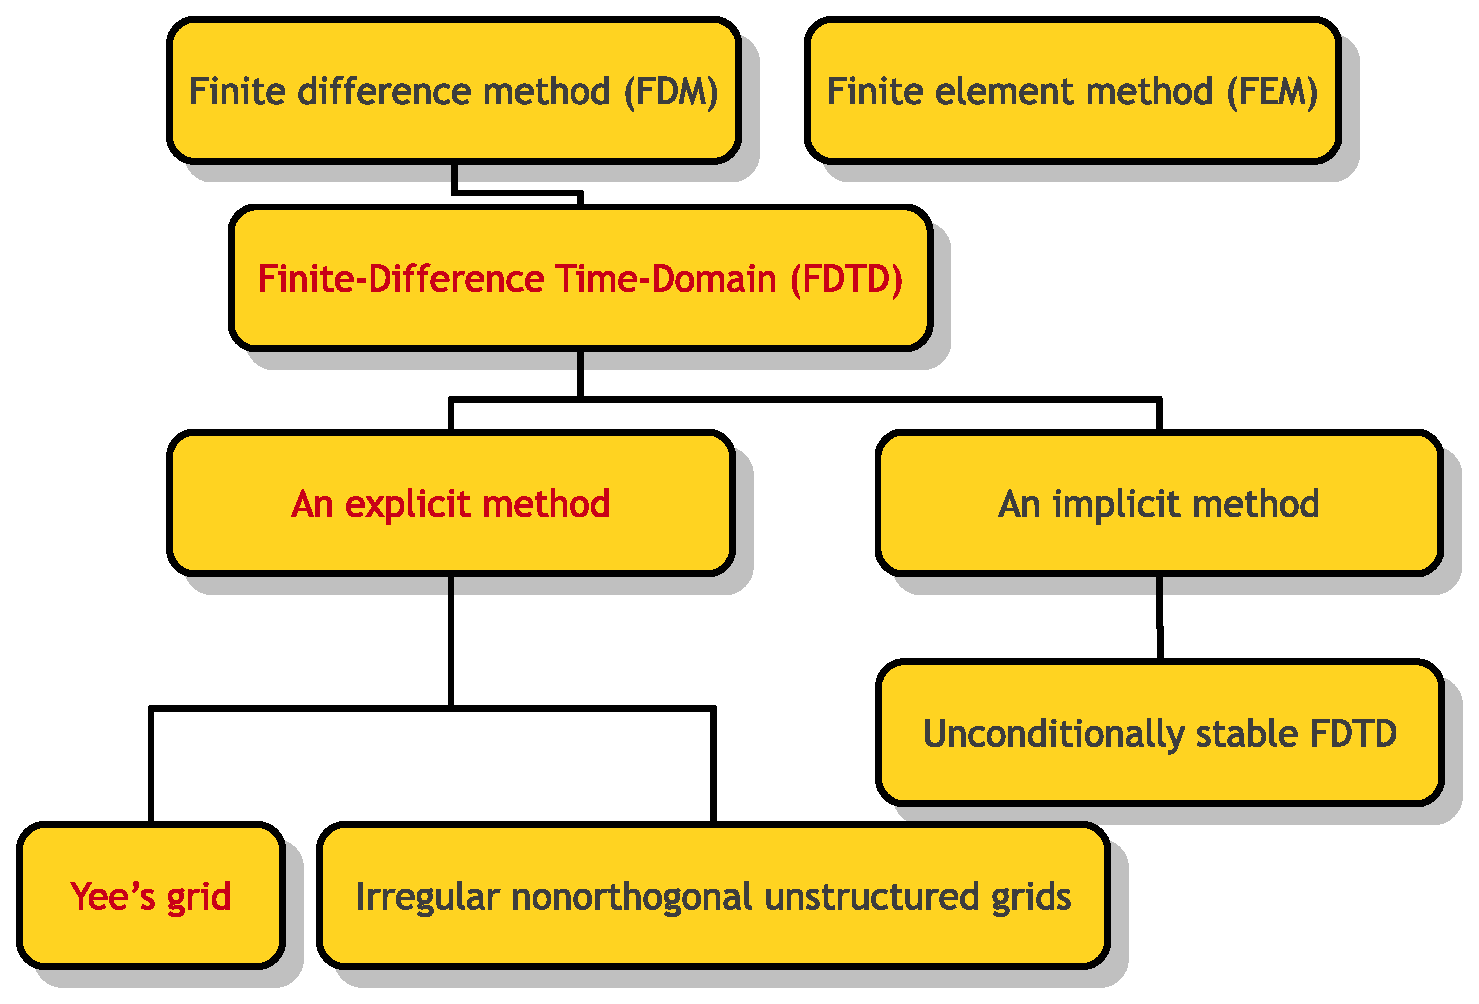
\includegraphics[width=\textwidth]{figure/class_nm}
  \caption{Classification of the numerical method in electrodynamics. GMES is an implementation of the explicit version of the FDTD method in the Yee's grid.}
  \label{fig:class_nm}
\end{figure}

The basic form of the FDTD\index{FDTD} with space grid and time-stepping was introduced by \citet{yee_numerical_1966}. The finite-difference forms are derived from the partial differential form of the Maxwell's equations\index{Maxwell's equations} with central-difference approximations\index{central-difference approximation} to the space and time differentials. The electric and magnetic field vectors in the resulting equations are solved in a leapfrog manner. The electric field vectors are solved at a given instant in time and then the magnetic field vectors are solved at the next instant in time.

The most noticeable advantages of FDTD\index{FDTD} is the easiness of algorithm. Users can easily understand how to use it and know what to expect from a given model. As a result, FDTD has a huge popularity over the past 20 years. According Wikipedia\footnote{\url{http://en.wikipedia.org/wiki/Finite-difference_time-domain_method}}, approximately 2,000 FDTD-related publications appeared in the science and engineering literature in 2006. Also, at 2008, there are at least 27 commercial/proprietary FDTD software vendors; 8 free-software/open-source-software FDTD projects; and 2 freeware/closed-source FDTD projects.

The FDTD\index{FDTD} method is preferred as a handy method. Because FDTD\index{FDTD} is a space-domain technique, users can set up the calculation domain, as like a real experimental setup. Various types of sources can be used to excite the fields. (non)linear, (non)dispersive, and gain or loss medium can be placed with any dimension and any shapes in the calculation domain. Because, the calculation domain of FDTD\index{FDTD} method is space-time domain, setting and analyzing the domain is much like that of real experiment. During the simulation, the $\mathbf{E}$ and $\mathbf{H}$ fields are calculated everywhere in the computational domain as they evolve in time, it lends itself to providing animated displays of the electromagnetic field movement through the model. This type of display is useful in understanding what is going on in the model, and to help ensure that the model is working correctly.

Like all the other numerical methods, FDTD\index{FDTD} also has disadvantages. Ironically, the origin of most noticeable advantage and disadvantage is the same, the discretization of space and time. The spatial grid must be sufficiently fine to resolve both the smallest electromagnetic wavelength and the smallest geometrical feature in the model, and hence very large computational domains can be developed, which results in very long solution times.

Most FDTD\index{FDTD} programs focus on this problem, and their designs are focused to overcome these disadvantages. However, we have focused on the advantages and try to reflect the advantages of the FDTD\index{FDTD} algorithm on the design and program. The difference in starting point of the development leads to the unique design of GMES\index{GMES}, the FDTD\index{FDTD} program we developed. FDTD\index{FDTD} itself is quite suitable to the object-oriented programming\index{object-oriented programming} (OOP\index{OOP}). The versatility characteristics of FDTD\index{FDTD} is represented in OOP\index{OOP}. The versatility of FDTD\index{FDTD} program is determined by the ability to represent the material type and shape. The current version of GMES\index{GMES} has full advantages on representing material types. However, the ability to represent accurate shape of the structure is planed in near future.

Of course, The speed and memory problem could not be neglected to make a pragmatic FDTD\index{FDTD} program. The na\"ive application of the OOP to the FDTD\index{FDTD} algorithm causes enormous memory consumption and very low calculation speed. The design should represent the characteristics of FDTD\index{FDTD} algorithm in efficient way. The design of GMES\index{GMES} in early stage was based on just simple na\"ive OOP scheme, but as it has become developed, GMES\index{GMES} could get sophisticated design with memory and calculation efficiency.

The main target of GMES\index{GMES} is a simulation for the plasmon device\index{plasmon device} though it can handle various optical device\index{optical device}. The plasmon device\index{plasmon device} is a nano-scaled device consisting of metals and dielectrics. Thus, we have given our special effort to represent dispersive medium in FDTD\index{FDTD} algorithm. As a result, GMES\index{GMES} has algorithms based on Drude-critical point model\index{Drude-critical point model} which can represent dispersive property of various metals accurately.

Since I registered the GMES\index{GMES} project in SourceForge\index{SourceForge} at 20th June 2006, GMES\index{GMES} has been downloaded over 1,000 times. GMES\index{GMES} has been developed only using open source programs and it is licensed in GNU\index{GNU} general public license\index{general public license} (GPL\index{GPL}) v3.0\footnote{\url{http://www.gnu.org/licenses/gpl.html}}. The number of lines in source code exceeds 30,000 lines and written in C\verb!++! and Python. GMES\index{GMES} operates on any Unix-like system and Windows\textsuperscript{\texttrademark}.

For interpretation of the references to color in the figures in this thesis, the reader is referred to the electronic version of this thesis. The PDF version of this thesis can be obtained from GIST library\footnote{\url{http://library.gist.ac.kr}} or national assembly library\footnote{\url{http://www.nanet.go.kr}}.
